\documentclass{standalone}

\usepackage{tikz}
\usetikzlibrary{angles,quotes}
\usepackage{amsmath,amssymb,amsfonts}

\usepackage{pgfplots}

\pgfplotsset{compat=newest}
\pgfplotsset{every axis/.append style={
                     tick label style={font=\footnotesize},
                 }}

\begin{document}
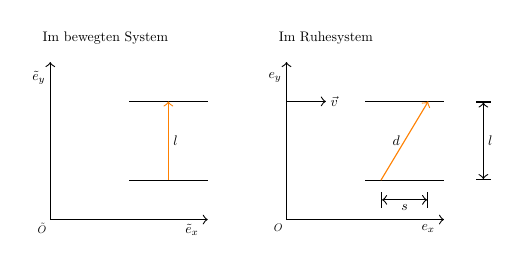
\begin{tikzpicture}
\draw (1.7,3.3) node[scale=0.5]{Im bewegten System};
\draw[->](1,1)--(3,1) node[pos=0.9,below,scale=0.5]{$\tilde{e}_x$};
\draw[->](1,1)--(1,3) node[pos=0.9,left,scale=0.5]{$\tilde{e}_y$};
\draw (1,1) node[scale=0.4,anchor=north east]{$\tilde{O}$};
\draw[-](2,1.5)--(3,1.5);
\draw[-](2,2.5)--(3,2.5);
\draw[->,color=orange](2.5,1.5)--(2.5,2.5) node[midway,right,scale=0.5,color=black]{$l$};

\draw (4.5,3.3) node[scale=0.5]{Im Ruhesystem};
\draw[->](4,1)--(6,1) node[pos=0.9,below,scale=0.5]{$e_x$};
\draw[->](4,1)--(4,3) node[pos=0.9,left,scale=0.5]{$e_y$};
\draw (4,1) node[scale=0.4,anchor=north east]{$O$};
\draw[->](4,2.5)--(4.5,2.5) node[pos=1,right,scale=0.5]{$\vec{v}$};

\draw[-](5,1.5)--(6,1.5);
\draw[-](5,2.5)--(6,2.5);
\draw[|<->|](6.5,1.5)--(6.5,2.5) node[midway,right,scale=0.5]{$l$};
\draw[->,color=orange](5.2,1.5)--(5.8,2.5) node[midway,left,scale=0.5,color=black]{$d$};
\draw[|<->|](5.2,1.25)--(5.8,1.25) node[midway,below,scale=0.5]{$s$}; 
\end{tikzpicture}
\end{document}